
\chapter{Dise�o de paquetes}

Este cap�tulo muestra c�mo se agrupan por cercan�a funcional y sem�ntica las clases y dem�s elementos del sistema en diferentes paquetes, que permiten su manipulaci�n en grupos. Se identificar�n los paquetes m�s
relevantes del sistema y se describir� su finalidad.

\section{Especificaci�n de los paquetes de la aplicaci�n}

Los paquetes en los que se puede descomponer el simulador, parte de los subsistemas que lo constituyen:


\begin{itemize}
 \item \textbf{Paquete es.uco.simAS}.
 \item \textbf{Paquete editor}.
 \item \textbf{Paquete simulador}.
 \item \textbf{Paquete util.gramatica}.
 \item \textbf{Paquete centroayuda}.
 \item \textbf{Paquete resources}.
\end{itemize}

\subsection{Paquete es.uco.simAS}

Este es el paquete general de la aplicaci�n y contiene a los dem�s paquetes. Al ser un proyecto de la \textit{Universidad de C�rdoba}, se ha seguido la recomendaciones de Java a la hora de nombrar los paquetes y se ha supuesto el dominio \textbf{es.uco.simAS} para nombrar este paquete.

\subsection{Paquete editor}

El paquete \textbf{editor} contiene todas las clases del editor de gram�ticas (tanto las de informaci�n como las que solamente contienen elementos gr�ficos). El paquete importa a los paquetes \textit{util.gramatica}, para hacer uso de las gram�ticas de contexto libre; \textit{centroayuda}, para interactuar con la ayuda; \textit{resources}, donde se almacenan todos los iconos y recursos gr�ficos para la interfaz; y el \textit{paquete del simulador}, lo importa para poder transferirle una gram�tica.

El paquete editor se puede ver en la figura \ref{paqeditor}.

\begin{figure}[H]
      \begin{center} 
	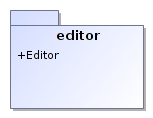
\includegraphics[scale=0.5]{img/paqeditor.jpg}
	\caption{Paquete editor}
	\label{paqeditor}
      \end{center}
  \end{figure}


\subsection{Paquete simulador}

El paquete \textbf{simulador} contiene todas las clases del simulador de gram�ticas (tanto las
de informaci�n como las que solamente contienen elementos gr�ficos). El paquete
importa a los paquetes \textit{util.gramatica}, para hacer uso de las gram�ticas de contexto
libre; \textit{centroayuda}, para interactuar con la ayuda; \textit{resources}, donde se almacenan
todos los iconos y recursos gr�ficos para la interfaz; y el \textit{paquete del editor}, lo importa para poder transferirle una gram�tica de vuelta.

El paquete simulador se puede ver en la figura \ref{paqsimulador}.

\begin{figure}[H]
      \begin{center} 
	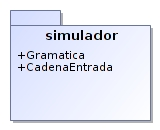
\includegraphics[scale=0.5]{img/paqsimulador.jpg}
	\caption{Paquete simulador}
	\label{paqsimulador}
      \end{center}
  \end{figure}

\subsection{Paquete util.gramatica}

Este paquete contiene todas las clases relacionadas con las gram�ticas de contexto
libre, adem�s de la clase que representa a las funciones de error. 

El paquete util.gramatica se puede ver en la figura \ref{paqgramatica}.

\begin{figure}[H]
      \begin{center} 
	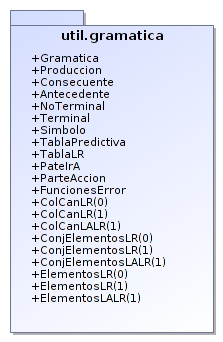
\includegraphics[scale=0.5]{img/paqgramatica.jpg}
	\caption{Paquete util.gramatica}
	\label{paqgramatica}
      \end{center}
  \end{figure}

\subsection{Paquete centroayuda}

Este paquete contiene la ventana del centro de ayuda y todos los recursos de
la ayuda de SimAS (todos los cap�tulos en formato html de la ayuda).

El paquete centroayuda se puede ver en la figura \ref{paqayuda}.

\begin{figure}[H]
      \begin{center} 
	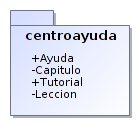
\includegraphics[scale=0.5]{img/paqayuda.jpg}
	\caption{Paquete centroayuda}
	\label{paqayuda}
      \end{center}
  \end{figure}

\subsection{Paquete resources}

Este paquete contiene todos los recursos gr�ficos utilizados por los componentes
de la interfaz gr�fica de SimAS (iconos, im�genes, tipos de letra, etc�tera). N�tese
que los componentes de la ayuda se han situado en el paquete \textit{centroayuda} en
lugar de hacerlo en este. As� se asegura que todos los recursos gr�ficos usados
por el programa est�n en el mismo paquete y separados de otros recursos que solo
usa un m�dulo concreto, como es el Centro de ayuda.

Este paquete aparece vac�o en el diagrama porque realmente no contiene
ninguna clase de las especificadas en el estudio del sistema, sino que contiene recursos gr�ficos de la interfaz
(que son demasiados como para enumerarlos en el diagrama).

\section{Diagrama de paquetes de la aplicaci�n}

En la figura \ref{dpaquetes} se muestra el diagrama de paquetes del simulador, seg�n
lo analizado anteriormente. N�tese que en los paquetes �nicamente se muestran los elementos
de informaci�n finales de la aplicaci�n (las clases que representan objetos de la
interfaz no se recogen en este diagrama, puesto que complicar�an en gran medida
su presentaci�n y comprensi�n).

 \begin{figure}[H]
      \begin{center} 
	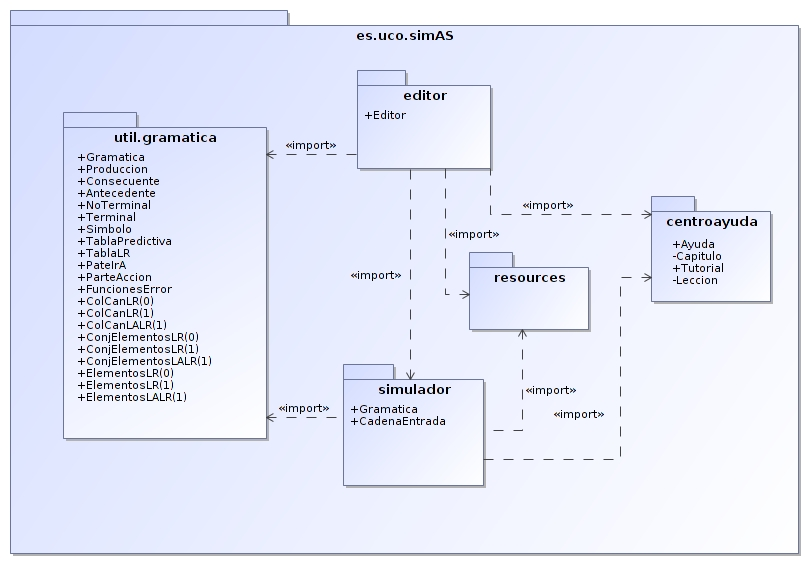
\includegraphics[scale=0.5]{img/paquetes.jpg}
	\caption{Diagrama de paquetes}
	\label{dpaquetes}
      \end{center}
  \end{figure}
